\documentclass[compress,aspectratio=43,11pt]{beamer}
\usepackage{ctex}
\usepackage{subcaption}
\usepackage{tikz}
\usetikzlibrary{shapes,arrows}
\usepackage{verbatim}
\usepackage{multimedia}

\pdfstringdefDisableCommands{  %hack the hyperref support CJK
\let\CJK@XX\relax
\let\CJK@XXX\relax
\let\CJK@XXXp\relax
\let\CJK@XXXX\relax
\let\CJK@XXXXp\relax
}

%------------ for headline theme--------------
%\begin{comment}   

\usetheme{Ilmenau}    %default, Antibes, Bergen, Berkeley, Boadilla, boxes, CambridgeUS, Darmstadt, Singapore, Luebeck,Ilmenau...
\useoutertheme{miniframes} %smoothbars, split, tree, default, infolines, miniframes, sidebar...
\usecolortheme{whale}
\useinnertheme{rectangles}

%\setbeamersize{mini frame size=0em}
%\setbeamersize{mini frame offset=1em}

\setbeamertemplate{frametitle}
{
  \vskip -0.455em     %set height position
  \begin{beamercolorbox}[ht=1.2em,wd=\paperwidth]{frametitle}   %set frametitle box
       \strut\insertframetitle\strut
  \end{beamercolorbox}
}

%\end{comment}
%------------ for headline theme--------------

%------------ for siderbar theme--------------
\begin{comment}   

\usetheme{Berkeley}    %default, Antibes, Bergen, Berkeley, Boadilla, boxes, CambridgeUS, Darmstadt, Singapore, Luebeck,Ilmenau...
\useoutertheme{sidebar} %smoothbars, split, tree, default, infolines, miniframes, sidebar...
\usecolortheme{whale}
\useinnertheme{rectangles}
% for side bar
\setbeamertemplate{frametitle}
{
  \vskip -0.535em     %set height position
  \begin{beamercolorbox}[height=1.2em,wd=1\paperwidth]{frametitle}   %set frametitle box
       \strut\Large\insertframetitle\strut
  \end{beamercolorbox}
}
\setbeamersize{sidebar width left=1.5cm}
\setbeamertemplate{headline}{} % swith the footline
\setbeamertemplate{siderbar left}{}

\makeatletter
  \setbeamertemplate{sidebar \beamer@sidebarside}%{sidebar theme}
  {
    \beamer@tempdim=\beamer@sidebarwidth%
    \advance\beamer@tempdim by -6pt%
    \insertverticalnavigation{\beamer@sidebarwidth}%
    \vfill
    \ifx\beamer@sidebarside\beamer@lefttext%
    \else%
      \usebeamercolor{normal text}%
      \llap{\usebeamertemplate***{navigation symbols}\hskip0.1cm}%
      \vskip2pt%
    \fi%
}%
\makeatother

\end{comment}
%------------ for siderbar theme--------------

%------------ for thesis theme--------------
\begin{comment}   
% for TorinoTh thesis
\usetheme[language=english,
titlepagelogo=logopolito,
bullet=circle,
pageofpages=of,
titleline=true,
color=blue
]{TorinoTh}

\definecolor{myblue}{RGB}{0,162,238}
\definecolor{myred}{RGB}{241,74,45}
\definecolor{mygreen}{RGB}{20,155,82}
\setbeamertemplate{frametitle}
{
  \vspace{-0.3em}
  \flushleft\insertframetitle{\centering{\vspace{-0.8em}\color{myblue}\hspace{0em}\rule{\columnwidth}{0.8pt}}}
}

\rel{��ʦ}
\ateneo{�Զ���}
\date{\today}
\end{comment}
%------------ for thesis theme--------------

\setbeamercovered{transparent}
\setbeamertemplate{footline}{} % swith the footline
%\setbeamertemplate{navigation symbols}{} % switch the symbols
%\logo{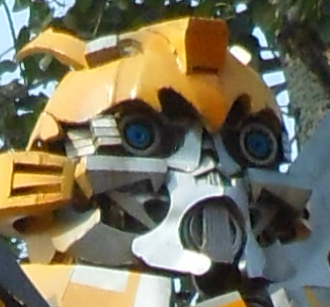
\includegraphics[height=0.8cm]{Pic}}

\title{My Beamer Template}
\author{HX wang}

\begin{document}
\frame[plain]{\titlepage}

\frame{\frametitle{Content}\tableofcontents[pausesections,hideallsubsections]\hypertarget{jumpToContent}{}}

\section{ {\heiti����}}

\frame{\frametitle{Content}\tableofcontents[currentsection]}

\frame{\sectionpage}

\begin{frame}{Introduction}
\heiti
\centering The introduction. ����Ҳ֧�֡�\\kankan

\end{frame}

\section{Basic}

\frame{\frametitle{Content}\tableofcontents[currentsection]}

\begin{frame}[<+- | alert@+>]{Overlap}
  \begin{itemize}
	\item<1- | alert@2> Item1\\
	  \fbox{
		\begin{minipage}{0.7\columnwidth}
		  \structure{Some thing about item1.}
		\end{minipage}}
	\item<1,3- | alert@3> Item2\\
	  \fbox{
		\begin{minipage}{0.7\columnwidth}
		  \structure{Some thing about item2.}
		\end{minipage}}
	\item<1,4- | alert@4>  Item3\\
	  \fbox{
		\begin{minipage}{0.7\columnwidth}
		  \structure{Some thing about item3.}
		\end{minipage}}
  \end{itemize}
\end{frame}

\begin{frame}[fragile,label=mycode]{Code}
  \footnotesize
	\begin{semiverbatim}
	  \uncover<1->{\alert<0>{int main (void)}}
	  \uncover<1->{\alert<0>{\{}}
	  \uncover<1->{\alert<1>{ \alert<4>{std::}vector<bool> is_prime (100, true);}}
	  \uncover<1->{\alert<1>{ for (int i = 2; i < 100; i++)}}
	  \uncover<2->{\alert<2>{ if (is_prime[i])}}
	  \uncover<2->{\alert<0>{ \{}}
	  \uncover<3->{\alert<3>{ \alert<4>{std::}cout << i << " ";}}
	  \uncover<3->{\alert<3>{ for (int j = i; j < 100;}}
	  \uncover<3->{\alert<3>{ is_prime [j] = false, j+=i);}}
	  \uncover<2->{\alert<0>{ \}}}
	  \uncover<1->{\alert<0>{ return 0;}}
	  \uncover<1->{\alert<0>{\}}}
	\end{semiverbatim}
  \uncover<4->{Note the use of \alert{\texttt{std::}}.}
\end{frame}

\begin{frame}[fragile]{Counter Intro}
	\begin{block}{Latex counter}
		\tiny
	\begin{verbatim}
		\newcounter{mycounter}  \\init to 0.
		\setcounter{mycounter}{value}   \\ set mycounter to value
		\addtocounter{mycounter}{value}   \\ mycounter + value, can be negtive.
		\themycounter \\ print mycounter out.
		\value{mycounter}  \\get the counter value, can be used in latex
		PS:  \newcounter method has global behave.
	\end{verbatim}
	\end{block}
	\begin{block}{Tex counterpart:}
		\tiny
	\begin{verbatim}
		\newcount\mycounter
		\mycounter <value>\relax
		\advance\mycounter <value>\relax
		\the\counter
		\counter
		PS: \newcount works locally
	\end{verbatim}
	\end{block}
	Latex counter is prefertable.
\end{frame}

\newcounter{mylocalcounter}
\begin{frame}{Counter example}
	\setcounter{mylocalcounter}{2}
	\begin{itemize}
		\item<\value{mylocalcounter}-> {kankan1 \stepcounter{mylocalcounter}}
		\item<\value{mylocalcounter}-> {kankan2 \addtocounter{mylocalcounter}{2}}
		\item<\value{mylocalcounter}-> {kankan4 }
	\end{itemize}
\end{frame}

\begin{frame}{PipleLine}
  \begin{columns}[T,totalwidth=0.7\columnwidth]
	\begin{column}{0.4\columnwidth}
	  \begin{block}{}
		Two\\lines\\more\\moree\\moreee\\moreee.
	  \end{block}
	\end{column}
	\begin{column}{0.1\columnwidth}
	  \onslide<2>{\vspace{2em} \color{blue} \LARGE $\Leftarrow$}
	\end{column}
	\begin{column}{0.4\columnwidth}
	  \begin{block}{}
		One line (but aligned).
	  \end{block}
	\end{column}
  \end{columns}

  \begin{columns}[T,totalwidth=0.7\columnwidth]
	\begin{column}{0.4\columnwidth}
	  \begin{center}
		\vspace{-1em} \color{blue} \LARGE $\Downarrow$ 
	  \end{center}
	\end{column}
  \end{columns}

  \begin{columns}[T,totalwidth=0.7\columnwidth]
	\begin{column}{0.4\columnwidth}
	  \begin{block}{}
		Two\\lines.
	  \end{block}
	\end{column}
  \end{columns}
\end{frame}

\begin{frame}{Picture}
  \begin{columns}
	\begin{column}{0.7\columnwidth}
		\begin{figure}
	  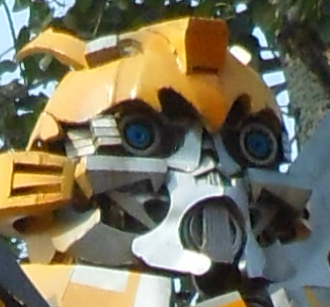
\includegraphics[width=1\columnwidth]{Pic}
		\end{figure}
	\end{column}
	\begin{column}{0.3\columnwidth}
	  \begin{block}{Figure}
		This is BB!
	  \end{block}
	  \begin{example}{Figure}
		This is example block.
	  \end{example}
	\end{column}
  \end{columns}
\end{frame}

\begin{frame}
\begin{center}
\begin{tikzpicture}
  \node (T) {text};
  \node (B) at (T.south east)[yshift=-30] {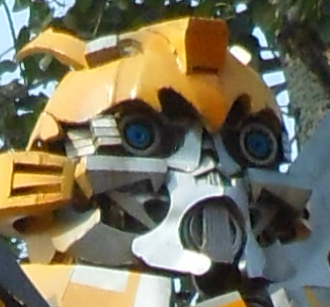
\includegraphics[width=0.1\columnwidth]{Pic}};
  \draw[->] (T) -- (B);
\end{tikzpicture}
\end{center}
\end{frame}

\begin{frame}{Three figures}
\newcommand{\mywidth}{0.3}

\setbeamercovered{invisible}
  \vspace{-3em}
  \flushleft��ͼ�п��Կ�����������ͼ��һ���ġ�
  \begin{figure}
	  \begin{subfigure}[t]{\mywidth\columnwidth}
	 \onslide<1->{ 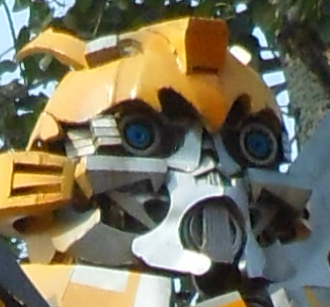
\includegraphics[width=1\columnwidth]{Pic}
	 \small\caption{This is Figure 1}}
	\end{subfigure}
	\begin{subfigure}[t]{\mywidth\columnwidth}
	\onslide<2->{  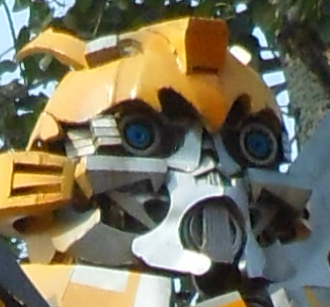
\includegraphics[width=1\columnwidth]{Pic}
	\caption{ͼ2}}
	\end{subfigure}
	\begin{subfigure}[t]{\mywidth\columnwidth}
	\onslide<3->{  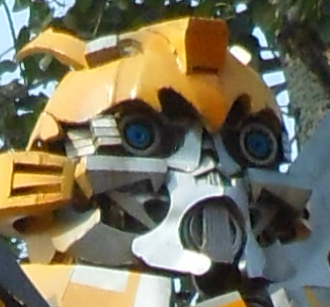
\includegraphics[width=1\columnwidth]{Pic}
	\caption{ͼ3}}
	\end{subfigure}
  \end{figure}
\end{frame}

\begin{frame}
	\begin{center}
		\begin{tikzpicture}
		\node[anchor=south west,inner sep=0] (image) at (0,0) {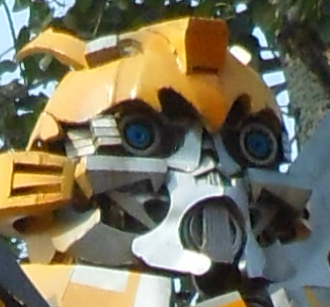
\includegraphics[width=0.8\textwidth]{Pic}};
			\begin{scope}[x={(image.south east)},y={(image.north west)}]
				\draw[help lines,xstep=.1,ystep=.1] (0,0) grid (1,1);
				\foreach \x in {0,1,...,9} { \node [anchor=north] at (\x/10,0) {0.\x}; }
				\foreach \y in {0,1,...,9} { \node [anchor=east] at (0,\y/10) {0.\y}; }

				\draw[red,ultra thick,rounded corners] (0.62,0.65) rectangle (0.78,0.75);
			\end{scope}
		\end{tikzpicture}
	\end{center}
\end{frame}

%\againframe{myoutlines}

\begin{frame}[shrink=20]{Graph1}
\tikzstyle{decision} = [diamond, draw, fill=blue!20, 
    text width=4.5em, text badly centered, node distance=3cm, inner sep=0pt]
\tikzstyle{block} = [rectangle, draw, fill=blue!20, 
    text width=5em, text centered, rounded corners, minimum height=4em]
\tikzstyle{line} = [draw, -latex']
\tikzstyle{cloud} = [draw, ellipse,fill=red!20, node distance=3cm,
    minimum height=2em]

\begin{tikzpicture}[node distance = 2cm, auto]
\node [block] (init) {initialize model};
    \node [cloud, left of=init] (expert) {expert};
    \node [cloud, right of=init] (system) {system};
    \node [block, below of=init] (identify) {identify candidate models};
    \node [block, below of=identify] (evaluate) {evaluate candidate models};
    \node [block, left of=evaluate, node distance=3cm] (update) {update model};
    \node [decision, below of=evaluate] (decide) {is best candidate better?};
    \node [block, below of=decide, node distance=3cm] (stop) {stop};
    % Draw edges
    \path [line] (init) -- (identify);
    \path [line] (identify) -- (evaluate);
    \path [line] (evaluate) -- (decide);
    \path [line] (decide) -| node [near start] {yes} (update);
    \path [line] (update) |- (identify);
    \path [line] (decide) -- node {no}(stop);
    \path [line,dashed] (expert) -- (init);
    \path [line,dashed] (system) -- (init);
    \path [line,dashed] (system) |- (evaluate);
\end{tikzpicture}
\end{frame}

\begin{frame}[plain]{Two picture}
  ����ͼ��
  \only<1>{
	\begin{figure}
	  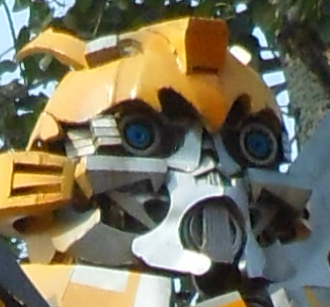
\includegraphics[width=0.6\columnwidth]{Pic}
	  \small\caption{Pic}
	\end{figure}
  }

  \only<2>{
	\begin{figure}
	  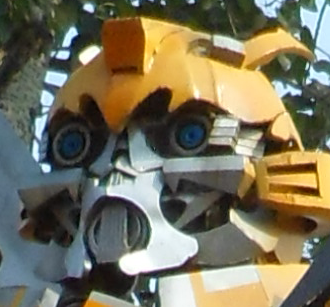
\includegraphics[width=0.6\columnwidth]{Pic2}
	  \small\caption{Pic2}
	\end{figure}
  }
  \end{frame}
  

\section{Conclusion}

\subsection{SubConclusion}

\frame{\frametitle{Content}\tableofcontents[currentsection]}

\frame{This is the beginning! Remember to make this note grown!\\\hyperlink{jumpToContent}{\beamergotobutton{Jump To Content}}}

\end{document}

%\usetheme{Warsaw} The full list of themes is:
%	  Antibes Bergen Berkeley Berlin Copenhagen Darmstadt Dresden Frankfurt Goettingen Hannover Ilmenau * JuanLesPins Luebeck Madrid Malmoe Marburg Montpellier PaloAlto Pittsburgh Rochester Singapore Szeged Warsaw boxes default 

%\usecolortheme{beaver} The full list of color themes is:
%	  default albatross beaver beetle crane dolphin dove fly lily orchid rose seagull seahorse whale wolverine

%\useoutertheme{infolines} Here is a list of all available outer themes:
%  infolines miniframes shadow sidebar smoothbars smoothtree split tree

%\useinnertheme{rectangles} Here is a list of all available inner themes:
%	  rectangles circles inmargin rounded

